% This file was converted to LaTeX by Writer2LaTeX ver. 0.5
% see http://www.hj-gym.dk/~hj/writer2latex for more info
\documentclass[a4paper]{report}
\usepackage[ascii]{inputenc}
\usepackage[T1]{fontenc}
\usepackage[english]{babel}
\usepackage{amsmath,amssymb,amsfonts,textcomp}
\usepackage{color}
\usepackage{array}
\usepackage{supertabular}
\usepackage{hhline}
\usepackage{hyperref}
\hypersetup{colorlinks=true, linkcolor=blue, citecolor=blue, filecolor=blue, pagecolor=blue, urlcolor=blue, pdftitle="Weather Radar Theory", pdfauthor=pfb, pdfsubject=, pdfkeywords=}
\usepackage[pdftex]{graphicx}
% Text styles
\newcommand\textstyleEmphasis[1]{\textit{#1}}
% Outline numbering
\setcounter{secnumdepth}{4}
\renewcommand\thesection{\arabic{chapter}.\arabic{section}}
\renewcommand\thesubsection{\arabic{chapter}.\arabic{section}.\arabic{subsection}}
\renewcommand\thesubsubsection{\arabic{chapter}.\arabic{section}.\arabic{subsection}.\arabic{subsubsection}}
\renewcommand\theparagraph{\arabic{chapter}.\arabic{section}.\arabic{subsection}.\arabic{subsubsection}.\arabic{paragraph}}
\makeatletter
\newcommand\arraybslash{\let\\\@arraycr}
\makeatother
% Figure numbering
\renewcommand{\thefigure}{\arabic{chapter}.\arabic{figure}}
\newcommand{\Section}[1]{\section{#1} \setcounter{figure}{1}}
% Footnote rule
\setlength{\skip\footins}{1.2mm}
\renewcommand\footnoterule{\vspace*{-0.18mm}\setlength\leftskip{0pt}\setlength\rightskip{0pt plus 1fil}\noindent\textcolor{black}{\rule{0.25\columnwidth}{0.18mm}}\vspace*{1.02mm}}
% Pages styles
\makeatletter
\newcommand\ps@NewChapter{
  \renewcommand\@oddhead{}
  \renewcommand\@evenhead{}
  \renewcommand\@oddfoot{}
  \renewcommand\@evenfoot{}
  \renewcommand\thepage{\arabic{page}}
}
\newcommand\ps@Standard{
  \renewcommand\@oddhead{}
  \renewcommand\@evenhead{}
  \renewcommand\@oddfoot{}
  \renewcommand\@evenfoot{}
  \renewcommand\thepage{\arabic{page}}
}
\newcommand\ps@FirstPage{
  \renewcommand\@oddhead{}
  \renewcommand\@evenhead{}
  \renewcommand\@oddfoot{}
  \renewcommand\@evenfoot{}
  \renewcommand\thepage{\arabic{page}}
}
\newcommand\ps@Contents{
  \renewcommand\@oddhead{}
  \renewcommand\@evenhead{}
  \renewcommand\@oddfoot{}
  \renewcommand\@evenfoot{}
  \renewcommand\thepage{\roman{page}}
}
\makeatother
\pagestyle{plain}
\setlength\tabcolsep{1mm}
\renewcommand\arraystretch{1.3}
\newcounter{Text}[section]
\numberwithin{equation}{chapter}
\renewcommand\theText{\thesection.\arabic{Text}}
\pagenumbering{arabic}
\renewcommand{\thepage}{\arabic{chapter}.\arabic{page}}

\title{Passive Weather Radar Theory}

\begin{document}
\maketitle
\date{January 2011}

\clearpage\setcounter{page}{1}
\thispagestyle{Contents}

\tableofcontents

\clearpage\setcounter{page}{1}
\thispagestyle{Contents}

\listoffigures

\clearpage\setcounter{page}{1}
\chapter[Project Purpose and Scope]{Project Purpose and Scope}
The primary objectives of this project is to build and instrument using GNURadio and an Ettus LLC USRP in order to evaluate the former and gain experience on both. A Passive Weather Radar has been chosen as the vehicle to these ends because it is expansive enough to exercise GNURadio and it has some chance of success.

\bigskip

The literature suggests that frequencies below L band reflect well from precipitation. With the introduction of Telstra's "Next G" cell phone net work a number of wide band signals from moderately powerful transmitters using 800 MHz to 900 MHz is available. These signals have the desirable characteristic of mimicking bandwidth limited white noise.

\bigskip

There is also some suggestion that air current eddies may be detectable at about 900 MHz using Doppler signals.

\bigskip

So the secondary objectives are to investigate the possibility of using the Telstra signals for examining these phenomenon with no particular expectation of success or failure.

\clearpage\setcounter{page}{1}
\chapter[Introduction]{Introduction}
\section{Definition}
Passive Radar is a system that has many of the same functionality as an
active radar system but achieves its goals without transmitting any
radio frequency energy. As a substitute for the energy transmitted by
an active radar a passive radar relies upon remote transmitters
illuminating the area of interest.

\bigskip

Weather \ radar relies on Rayleigh scattering of radio frequency energy
by water droplets. Existing active weather radars are typically pulsed
Doppler radars using a wavelength of 10cm (S band).

\section{Basic Active Radar Theory}
Active radar works by transmitting a short pulse through a directional
antennae and receiving any subsequent reflections via the same antenna.
The antenna is then rotated to point in a new direction and \ the
process repeated. Figure \ref{fig:01} shows a typical transmission and reception of an active radar.

\begin{figure}
\centering 
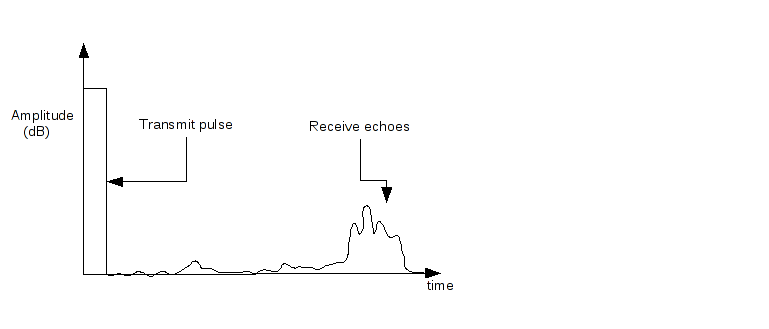
\includegraphics{Passive-Weather-Radar-Theory-fig-01.png}
\caption[Time series of an active radar signal]{Time series of an active radar signal}
\label{fig:01}
\end{figure}

\bigskip

The range aperture in the radial axis is a function of the transmit pulse
width and the aperture in the circumferential axis is a function of the
beam width formed by the directional antenna. The transmit function can be considered an approximation to a Dirac function $\delta(t)$ in time and the closer the approximation to the ideal the better the range resolution. However, resolution of Doppler values requires a wider transmit pulse so there is a design trade off to be made here. 

\begin{figure}
\centering 
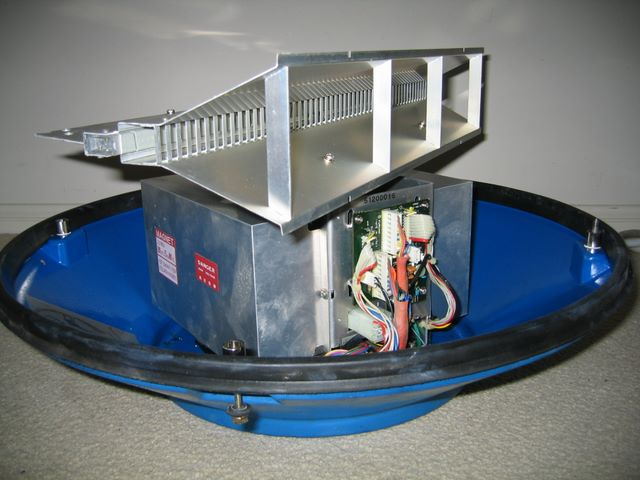
\includegraphics[scale=.75]{marine_radar_010.jpg}
\caption[Marine radar antenna consisting of a rotating slotted wave guide]{Marine radar antenna consisting of a rotating slotted wave guide}
\label{fig:slotted_wave_guide}
\end{figure}

In practice the antenna
is made to turn at a constant rate and the transmitter is made to
transmit at a constant repetition rate. The returned radio frequency
energy is converted to baseband where signal processing occurs and is
then presented to a PPI display for viewing or an A/D converter for
further processing (in which case the analog signal processing is,
typically, minimal). 

\bigskip

\textstyleEmphasis{\textup{In addition to signals of interest the return
is typically contaminated with unwanted artifacts such as ground
clutter. A large amount of this noise may be removed by using Doppler
processing in order }}\textstyleEmphasis{\textup{to
}}\textstyleEmphasis{\textup{remove those echoes having a velocity less
than some minimum value. In addition the velocity of the returns has
significant value in the context of a weather radar. Of course only
velocities along }}\textstyleEmphasis{\textup{the radial axis can be
observed.}} 

\bigskip

\textstyleEmphasis{\textup{The geometry of an active radar system when
the transmitter and the receiver antennas are co
}}\textstyleEmphasis{\textup{located (as they invariably are) is that
of radials intersecting co located circles. }}

\begin{figure}
\centering 
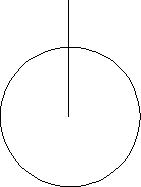
\includegraphics{Passive-Weather-Radar-Theory-fig-02.png}
\caption[Geometry of an active radar system in the horizontal plane]{Geometry of an active radar system in the horizontal plane}
\label{fig:02}
\end{figure}

\section{Basic Passive Radar Theory }
\textstyleEmphasis{\textup{Because passive radar relies upon
transmitters of opportunity the receiver and signal processing must be
designed to suit the available illumination. However the transmitter
and receiver are very unlikely to be co located so the geometry is
possibly not going to be the same as the in the case of an active
radar. In general a passive radar will be made to receive the
transmission signal and the delayed reflected signals in order to
identify targets of interest. As in the case of the active radar, and
knowing the frequency and pseudo phase of the transmitter, Doppler
processing may be employed. In general geometrical and receiver dynamic
range considerations will require the more than one transmitter be
used.}} 

\bigskip

There is an analog between active and passive radars with respect to the range and Doppler resolutions including the trade off between the precision of the two.

\bigskip

\textstyleEmphasis{\textup{There are two realizable implementations of a
passive radar. One involves a directional beam pattern
}}\textstyleEmphasis{\textup{for the receiver which can be made to
point in a certain direction. Each transmitter forms an elliptical
isovalue with the transmitter and receiver as foci. Another measures
the difference in time (and, hence, distance) between the direct
arrival of the transmitter signal and the reflected signal in order to
form an ellipse with foci at the transmitter and receiver upon which
the target must lie. In this case the available degrees of freedom is
equal to the number of transmitters.}}

\clearpage\setcounter{page}{1}
\chapter[Design Decisions]{Design Decisions}
\section[Decisions on the Measurement Method]{Decisions on the Measurement Method}
\textstyleEmphasis{\textup{The most
basic}}\textstyleEmphasis{\textbf{\textup{
}}}\textstyleEmphasis{\textup{decisions to be made are those concerning
the measurement method. These decisions will drive other decisions such
as the number of receivers required and the processing chains.}}

\bigskip

\textstyleEmphasis{\textup{A key decision is the illumination source. It
is proposed to use the Telstra Next G {\textquotedblleft}Upper 800 MHz
Band{\textquotedblright} signals. These signals emanate from
Telstra{\textquotesingle}s cell phone towers. They are Direct Spread
Spectrum signal of about 10 MHz wide in the 880 MHz to 890 MHz band.
This bandwidth will yield a resolution in the order of 30 meters. It
may be possible to supplement illumination from this band with
illumination from Telstra{\textquotesingle}s {\textquotedblleft}Lower
800 MHz Band{\textquotedblright} signals. These occupy the band from
\ 810 MHz to 820 MHz.}}

\bigskip

\textstyleEmphasis{\textup{Another key decision is to answer the
question, {\textquotedblleft}should the direction from the receiver to
the target }}

\bigskip

\textstyleEmphasis{\textup{be measured and, if so,
how{\textquotedblright}? Measuring the angle imposes difficulties but
yields an extra degree of freedom so that it will be possible to get
target estimates from just one transmitter. However, it may be
necessary to drop this requirement and fall back on a time difference
or pseudo time zero scheme.}}

\subsection[Direction Measuring]{\textstyleEmphasis{\textup{Direction
Measuring}}}
\subsubsection[Mechanical]{\textstyleEmphasis{\textup{Mechanical}}}
\textstyleEmphasis{\textup{Measuring the direction by mechanical means
involves building a parabolic dish antenna mounted on a turntable. This
is difficult to implement, complex, possibly unreliable and potentially
dangerous to operate. This solution is rejected out of hand on these
grounds.}}

\subsubsection[Electronic]{\textstyleEmphasis{\textup{Electronic}}}
\textstyleEmphasis{\textup{There are at least two electronic methods to
estimate direction which may be employed}}

\subsubsection[Phased Array]{Phased Array}
\textstyleEmphasis{\textup{A phased array consists of a matrix of
regularly spaced simple antennae on a plane surface. Each antenna is
connected to its own receiver. The advantage of a phased array is a
super abundance of data and, if the matrix is more than one row, the
ability to measure elevations and direction in the horizontal plane.
This disadvantage is that it requires a lot of receivers and is
expensive. This solution is rejected because of the cost.}}

\subsubsection[Phase Interferometry]{Phase Interferometry}
If two simple antennae are place on a plane
separated by a distance with a wave front incident at a certain angle
then the path difference between the target is a function of that angle
and is represented by a phase difference between the antennae. \ For
unambiguous results the distance should be less than, or equal to, one
half the wavelength of the incident signal. However, two antennae
located so close together will almost certainly mutually couple and
distort the phase measurement of each. A possible solution to this problem is to measure the phase difference not of the 889 Mhz carrier frequency but the 10 MHz chip frequency used to directly spread the carrier. In this case the half wavelength spacing is about 15 meters.

\bigskip

\textstyleEmphasis{\textup{Elevation data can be measured in a similar
manner by placing a third antenna in the vertical plane. As with the
Phased Array approach Phased Interferometry requires one receiver per
antenna.}}

\bigskip

\textstyleEmphasis{\textup{The supper abundance of data that exists in
the Phased Array does not exist in this arrangement. Phase
Interferometry is sensitive to poor signal to noise.}}

\bigskip

Phase Interferometry provides angle information at a relatively cheap hardware cost.

\section[Omni-Direction Measuring]{Omni-Directional Measuring}
For this solution a minimum of one antenna
and receiver are required. 
The tracking geometry is an ellipse intersected by a line 
per transmitter. A minimum of two transmitters are required
for an unambiguous position determination.

\bigskip

\textstyleEmphasis{\textup{Elevation determination will probably not be
realistically achievable unless a Phase Interferometry is implemented
in the vertical plane. In addition, due to the non regular geometry the
30 meter resolution from a 10 MHz bandwidth will not be achievable
making higher bandwidth more important.}}

\bigskip

This solution is one of the the cheapest of solutions in terms of hardware.

\clearpage\setcounter{page}{1}
\chapter[Signal Processing]{Signal Processing}

\begin{figure}
\centering 
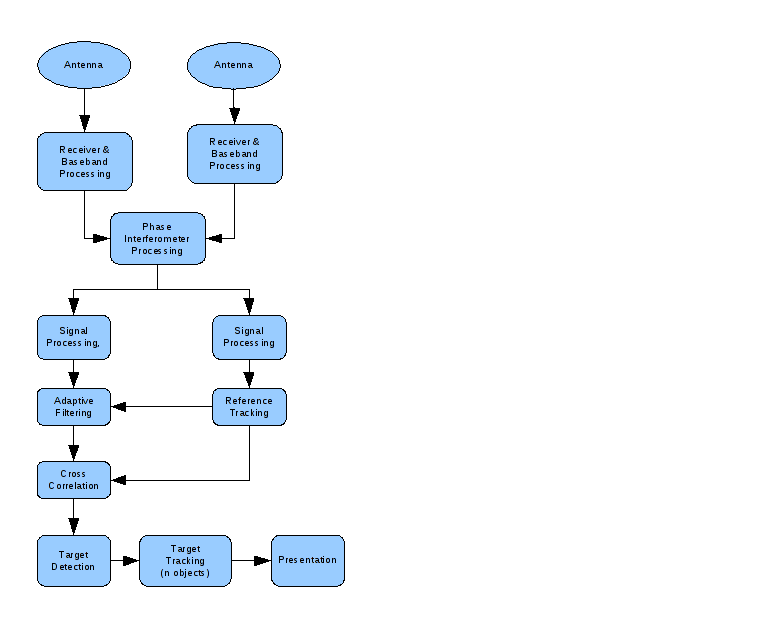
\includegraphics{Passive-Weather-Radar-Theory-fig-03.png}[h!]
\caption[Signal Processing Block Diagram]{Signal Processing Block Diagram}
\label{fig:03}
\end{figure}

\section[Major Signal Processing Blocks]{\textstyleEmphasis{\textup{Major Signal Processing Blocks}}}
\subsubsection[Receiver and Baseband Processing]{\textstyleEmphasis{\textup{Receiver and Baseband
Processing}}}

\begin{figure}
\centering 
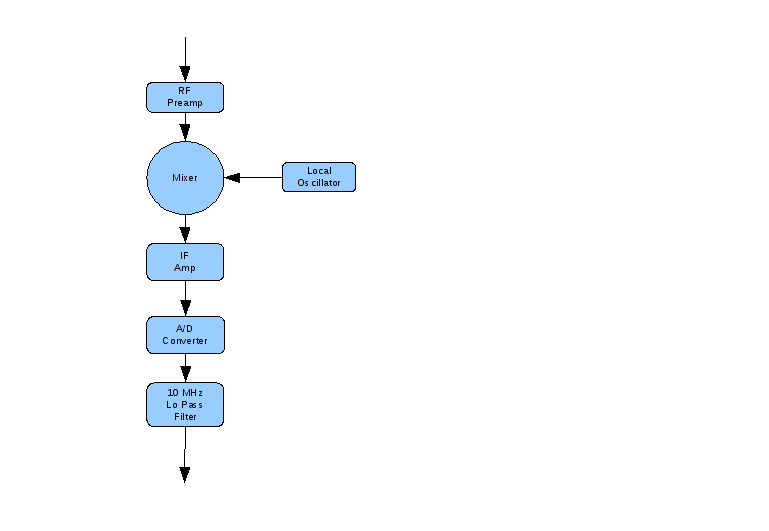
\includegraphics{Passive-Weather-Radar-Theory-fig-04.png}
\caption[Receiver and Baseband Processing]{Receiver and Baseband Processing}
\label{fig:04}
\end{figure}

\textstyleEmphasis{\textup{This block is wholly implemented in the USRP using the FPGA and analog hardware. As can be seen from figure \ref{fig:04} this block is a conventional single conversion receiver. The real and imaginary values produced by the mixer are digitized by the analog to digital converter in order to preserve the phase information.}}

\subsection[Phase Interferometer Processing]{Phase Interferometer Processing}

%\begin{figure}
%\centering 
%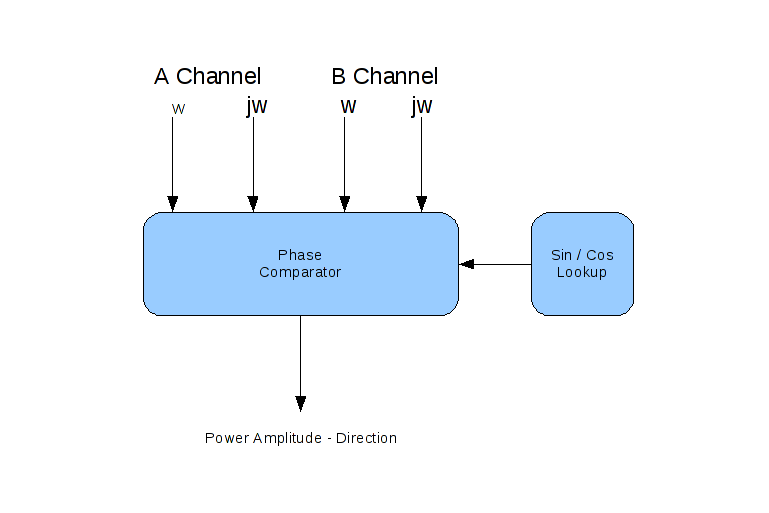
\includegraphics{Passive-Weather-Radar-Theory-fig-05.png}
%\caption[Phase Interferometer Processing]{Phase Interferometer Processing}
%\label{fig:05}
%\end{figure}

\textstyleEmphasis{\textup{This block develops a stream of $ \begin{bmatrix} S & \Theta \end{bmatrix} $.}}

\subsection[Adaptive Filtering]{Adaptive Filtering}

\begin{figure}
\centering 
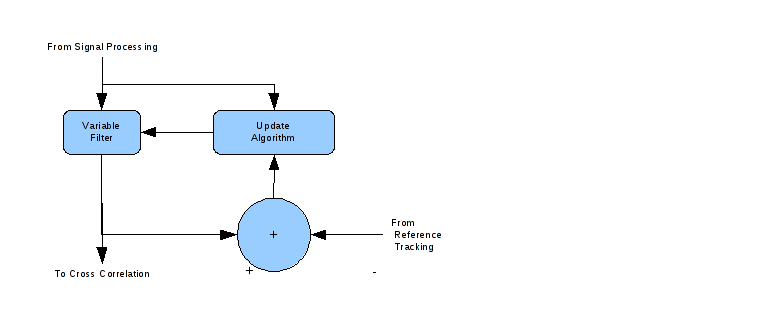
\includegraphics{Passive-Weather-Radar-Theory-fig-06.png}
\caption[Adaptive Filtering Block]{Adaptive Filtering Block}
\label{fig:06}
\end{figure}

The purpose of the Adaptive Filtering process is to remove the transmitter signal from the input. It uses an input from the Reference Tracking block as a reference of the signal to be removed.

\bigskip

As can be seen from figure \ref{fig:06} the filter is a standard FIR type. The Update Algorithm is made to update the tap coefficients in order to filter out the transmitter signal.

\subsection[Reference Tracking]{Reference Tracking}
The purpose of the Reference Tracker is to track all transmitters of interest and, possibly, reconstruct transmitter signals if necessary. Transmitters need to be tracked in order to develop time zero signals and to present references to the Adaptive Filter and the Cross Correlation blocks.

\subsection[Cross Correlation]{Cross Correlation}
The purpose of this block is to perform conventional cross correlations between transmitter reference signals and the filtered received echoes. The cross correlator acts as a matched filter and will provide processing gain. The intention is to aim for 50 dB of processing gain in this procedure.

\bigskip

Estimates of bistatic range and Doppler velocity will be developed in this block.

\subsection[Target Selection]{Target Selection}
The purpose of this block is to plot the
received correlated echoes using the appropriate geometry onto a
regular grid and to use the accumulated result to detect targets.
Target detection will use the Constant False Alarm Rate (CFAR)
algorithm. A user probability setting will be implemented.

\bigskip

\subsection[Target Tracking]{Target Tracking}
State information for targets is developed by
the Target Tracking block. Each target will be represented by an object
which implements a Kalman Filter.


\clearpage\setcounter{page}{1}
\chapter[Implementation]{Implementation}
In order to detect valid signals from the clutter it is important to maximize the processing gain and SNR. This chapter investigates the Matched Filter which is the block which will achieve this.

\bigskip

In this paper range refers to the sum of the distances from the transmitter to the target and from the target to the receiver and velocity refers to the rate of change to the range.

\section[Matched Filter Receivers]{Matched Filter Receivers}

The output of the Matched Filter $M(\tau, \phi)$ is:

\begin{equation}
M(\tau, \phi) = \frac{1}{T} \int_0^T x_r(t)x_t^*(t + \tau)e^{-i\phi t}dt
\label{eqn:matched_filter_analog}
\end{equation}
where

$T$ = the radar integration time, a constant, in seconds

$x_r(t)$ = the received signal

$x_t^*(t + \tau)$ = the complex conjugate transmitted signal

$\tau$ = the delay induced by the sum of the ranges from the transmitter to the receiver via the target

$\phi$ = the Doppler frequency induced by the sum of the velocities from the transmitter to the receiver via the target.

\bigskip

In practice a matched filter is usually implemented digitally in which case $x_r(t)$ and $x_t(t)$ are converted into digital signals $x_r[n]$ and $x_t[n]$ where $x[n] = x(nT_s)$ and $T_s$ is the constant sample period. In discrete form the output is:

\begin{equation}
M(\tau, \phi) = \frac{1}{N} \sum_{n=1}^{N} x_r[n] x_t^*[n + \tau]e^{-i\phi n}
\label{eqn:matched_filter_discrete}
\end{equation}
where

$N$ = the number of samples in the integration time ($T_sN = T$)

\bigskip

It is evident from equations \ref{eqn:matched_filter_analog} and \ref{eqn:matched_filter_discrete} that the expression for a matched filter is the Fourier Transform in $\phi$ of the correlation between the received signal and the transmitted signal delayed by time $\tau$.

\bigskip

If the noise corrupting the received signal is additive white Gaussian the following strategy will give the optimal target detection:

\begin{itemize}
\item{From the received signal $x_r(t)$, and a copy of the transmitted signal, $x_t(t)$, calculate $M(\tau, \phi)$.}
\item{Calculate the magnitude, $|M(\tau, \phi)|^2$.}
\item{Compare this quantity to some threshold, $l$. A target is indicated by $|M(\tau, \phi)|^2 > l$ at time delay $\tau$ and Doppler shift $\phi$.}
\end{itemize}

\section[The Ambiguity Function]{The Ambiguity Function}
Passive Radars are reliant on transmissions of opportunity and the maximum information that may be extracted from a signal from a target is encapsulated in these transmissions. It is useful to characterize the available transmissions. This is the purpose of the ambiguity function $\chi(\tau, \phi)$.

\begin{equation}
\chi(\tau, \phi) = \frac{1}{T} \int_0^T x(t)x^*(t + \tau)e^{-i\phi t}dt
\label{eqn:ambiguity_analog}
\end{equation}

As can be seen from equation \ref{eqn:ambiguity_analog} the ambiguity function describes how correlated a transmitter signal is with itself delayed by $\tau$ and shifted by Doppler $\phi$. It is also known as the time frequency autocorrelation function.

The discrete form of equation \ref{eqn:ambiguity_analog} is:

\begin{equation}
\chi(\tau, \phi) = \frac{1}{N} \sum_{n=1}^N x[n]x^*[n + \tau]e^{-i\phi n}
\label{eqn:ambiguity_discrete}
\end{equation}

It has been recognized that the ambiguity function of a transmission signal should have certain properties in order to be of use. These are due to factors such as the transmitted signal processing positive finite energy and that the signal cannot occupy a point in time and frequency. The most important of these properties are:

\begin{itemize}
\item{The maximum magnitude of the ambiguity function is a maximum at the origin. That is,

\begin{equation}
|\chi(0, 0)| \geq |\chi(\tau, \phi)|
\end{equation}}
\item{The magnitude of the ambiguity function is symmetric about the line $\tau = \phi$. That is,

\begin{equation}
|\chi(\tau, \phi)| = |\chi(-\tau, -\phi)|
\end{equation}}

\item{$|\chi(0, 0)|^2|$ is equal to the the amount of energy of the transmitted signal in the integration time. That is,

\begin{equation}
|\chi(0, 0)|^2 = \int_0^T |x(t)|^2 dt
\end{equation}}

\item{The volume under the surface described by $|\chi(\tau, \phi)|^2$ is equal to the energy in the transmitted signal. That is,

\begin{equation}
\int_0^T \int_0^T|\chi(\tau, \phi)|^2 d\tau d\phi = \left[\int_0^T |x(t)|^2 dt \right]^2
\end{equation}}
\end{itemize}

These necessary properties limit the possible ambiguity functions and, so, the possible transmitter signals. Any transmitter signal available is certainly going to be a compromise between the above properties.

\section[Resolution]{Resolution}
\label{sec:Resolution}

In order to optimally detect a target which produces time delay, $\tau$, and Doppler shift, $\phi$, it is necessary to maximize the value of $|\chi(0, 0)|^2$. Also, in order to minimize the detection of false targets it is necessary to minimize the value $|\chi(\tau, \phi)|^2$ for $(\tau, \phi) \ne (0, 0)$. Therefore the ideal transmitter signal is one that yields the ambiguity function so that:

\begin{equation}
|\chi_{ideal}(\tau, \phi)|^2 = 
\begin{cases}
1 & \text{if } (\tau, \phi) = (0, 0)\\
0 & \text{if } (\tau, \phi) \ne (0, 0)
\end{cases}
\end{equation}

This is the Dirac function in $\tau$ and $\phi$, $\delta(\tau, \phi)$, and is not realizable in practice (and is not a function).

\bigskip

More significantly if the transmitter signal approximates bandwidth limited white noise as DSS does then when $N$ is large (in normalized form):

\begin{equation}
|\chi(\tau, \phi)|^2 =
\begin{cases}
1 & \text{if } (\tau, \phi) = (0,0)\\
\frac{1}{TB} & \text{if } (\tau, \phi) \ne (0, 0)
\end{cases}
\label{eqn:TB}
\end{equation}
where

$T$ = the radar integration time in seconds

$B$ = the signal bandwidth in Hz

\bigskip

Equation \ref{eqn:TB} resembles an autocorrelation function squared. That is the best realizable ambiguity function has a spike at the origin and a surrounding floor. It follows that any signal having an amplitude less than $1/TB$ of the strongest signal cannot be detected. This relationship has significance when receiving signal having a wide range of energy amplitudes such as the direct signal from the transmitter and the targets. For instance with an integration time of 1 second and a bandwidth of 10 MHz the Matched Filter has a dynamic range of 
\begin{math}
|\chi(\tau, \phi)|^2 = 10 \log{\left(\frac{1}{1 * 10^6}\right)} = -70dB
\end{math}
with respect to the strongest signal.


\begin{figure}
\centering 
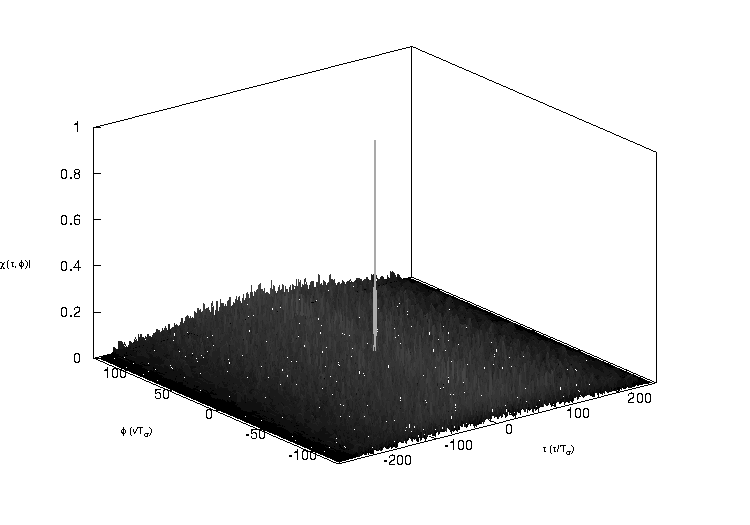
\includegraphics{Passive-Weather-Radar-Theory-fig-10.pdf}
\caption[Ambiguity function of white Gaussian noise]{Ambiguity function of white Gaussian noise}
\label{fig:10}
\end{figure}

\begin{figure}
\centering 
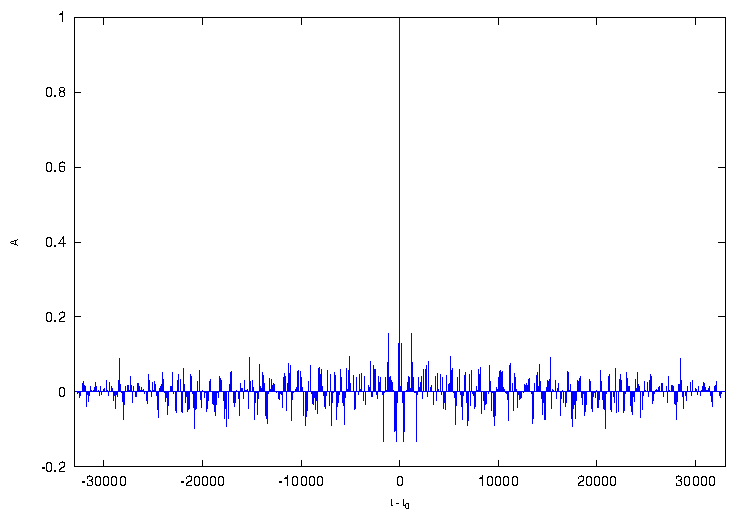
\includegraphics{Passive-Weather-Radar-Theory-fig-11.pdf}
\caption[white Gaussian noise autocorrelation]{white Gaussian autocorrelation}
\label{fig:11}
\end{figure}

\begin{figure}
\centering 
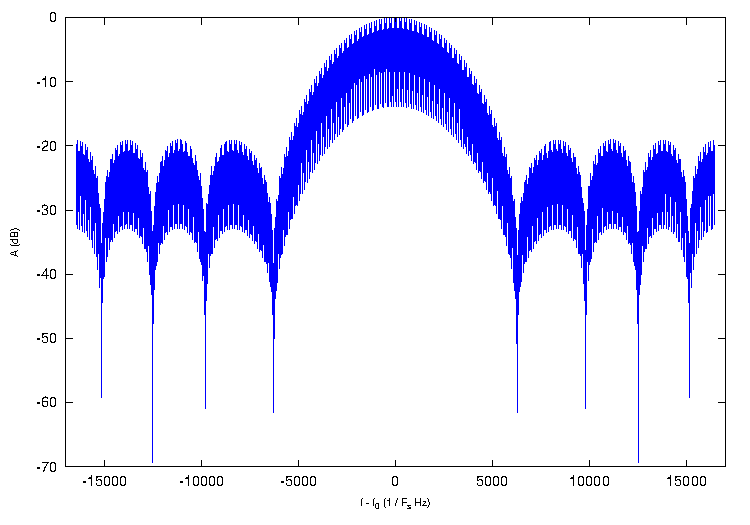
\includegraphics{Passive-Weather-Radar-Theory-fig-12.pdf}
\caption[white Gaussian noise envelope]{white Gaussian noise envelope}
\label{fig:12}
\end{figure}

\bigskip

Figure \ref{fig:10} shows a typical ambiguity function of a white Gaussian noise source. Notice the narrow spike at the origin and the surrounding noise floor. The amplitude ratio between the spike and the floor is improved by increasing the time bandwidth product. Figures \ref{fig:11} and \ref{fig:12} show the autocorrelation function and power or energy spectrum for the white noise source associated with \ref{fig:10}. Note the good autocorrelation characteristic and the $sinc^2()$ shape of the power function, both of which are typical of a source of this type.

\bigskip

Referring to figure \ref{fig:03} it can be seen that the input to the Cross Correlation Block is from the Adaptive Filtering Block. It is proposed that this latter block in conjunction with the Reference Tracking Block will attenuate the transmitter signal with respect to the echoes and so increase the dynamic range of the Cross Correlation Block. Further it will probably be necessary to shield the antennae in the direction of the transmitter in order to attenuate this signal even further although the advantage of this measure is to maximize the dynamic range of the analog portion of the receiver in order not to overload it.

\section[Implementation Problems]{Implementation Problems}
Typically Passive Radar processing is done digitally and, in fact, cannot, now days, be done practically done using analog techniques. The digital nature of the processing imposes its own set of problems.

\bigskip

Digital implementation of the Matched Filter is given by equation \ref{eqn:matched_filter_discrete}. The signals $x_r[n]$ and $x_t[n]$ are received and sampled at discrete points in time $nT_s$ where $T_s$ is the constant sampling period. Therefore $\tau$ is only defined at periods $T_s$ seconds. Likewise $\phi$ is only defined at multiples of $1/(NT_s)$ Hz. These two factors limit the resolutions of $\tau$ and $\phi$ and these limits are a function of $T_s$ and $N$. This corresponds to resolutions of $cT_s$ meters and $c/(NT_sf_c)$ Hz where $c$ is the speed of light and $f_c$ is the center frequency of the transmission.

\bigskip

Increasing the sampling frequency, $F_s$, and $NT_s$ decrease the granularity of the discrete representation of $M(\tau, \phi)$ in the respective domains. However, it is pointless to decrease these granularities such that the peak at the origin occupies a large number of $(\tau, \phi)$ cells. In this way $T_s$ and $N$ are tied to the function of merit, the ambiguity function $\chi(\tau, \phi)$, of the transmitter's signal.

\section[Radar Equation]{\textstyleEmphasis{\textup{Radar Equation}}}
The power  $P_{\tau }$ returning to the receiving antenna is given by
the radar equation:

\begin{equation}
P_{\tau }=\frac{P_{t}G_{t}A_{\tau }\sigma F^{4}}{\left(4\pi^{2}\right)R_{t}^{2}R_{\tau }^{2}}
\end{equation}
\textstyleEmphasis{\textup{where}}

 $P_{t}$\textstyleEmphasis{\textup{= transmitter power}}

 $G_{t}$\textstyleEmphasis{\textup{= gain of the transmitting antenna}}

 $A_{\tau }$\textstyleEmphasis{\textup{= effective aperture of the
receiving antenna}}

 $\sigma $\textstyleEmphasis{\textup{= radar cross section, or
scattering coefficient, of the target}}

 $F$\textstyleEmphasis{\textup{= pattern propagation factor}}

 $R_{t}$\textstyleEmphasis{\textup{= distance between the transmitter
and the target}}

 $R_{\tau }$\textstyleEmphasis{\textup{= distance between the
target and the receiver}}

\bigskip

\textstyleEmphasis{\textup{For atmospheric targets the pattern
propagation factor will consist mainly of the path loss. The path loss
in rural areas }}$L_{O}$\textstyleEmphasis{\textup{(in dB) is given by
the Hata Model for Open Areas:}}

\begin{equation}
L_{O}=L_{U}-4.78\left(\log (f)\right)^{2}+18.33\log (f)-40.94
\end{equation}
\textstyleEmphasis{\textup{where}}

 $L_{U}$\textstyleEmphasis{\textup{= path loss in urban areas in dB}}

 $f$\textstyleEmphasis{\textup{= frequency in MHz}}

\bigskip

\textstyleEmphasis{\textup{In turn the path loss in urban areas }}
$L_{U}$ \textstyleEmphasis{\textup{is given by the Hata Model for Urban
Areas:}}

\begin{equation}
L_{U}=69.55+26.16\log (f)-13.82\log (h_{t})-C_{H}+\left(44.9-6.55\log(h_{t})\right)\log (R_{t}+R_{\tau })
\end{equation}
\textstyleEmphasis{\textup{where the antenna height correction factor $C_{H}$ is given by:}}

\begin{equation}
C_{H}=0.8+\left(1.1\log (f)-0.7\right)h_{\tau}-1.56\log (f)
\end{equation}
where

 $f$= transmission frequency in MHz

 $h_{t}$= height of transmitter antenna

 $h_{\tau}$= height of receiver antenna

 $R_{t}$= distance between the transmitter and the target

 $R_{\tau }$= distance between the target and the receiver

\bigskip

A simpler approximation for the path loss, $L$, between two isotropic antennae is:

\begin{equation}
L=20 log\left(\frac{4 \pi \left(R_{t} + R_{\tau}\right)}{\lambda}\right)
\end{equation}
where

 $R_{t}$= distance between the transmitter and the target in meters

 $R_{\tau}$= distance between the target and the receiver in meters

 $\lambda$= wavelength of the transmission in meters

\section[Hardware]{\textstyleEmphasis{\textup{Hardware}}}
\subsection[Universal Software Radio Peripheral (USRP)]{Universal Software Radio Peripheral (USRP)}

\begin{figure}
\centering 
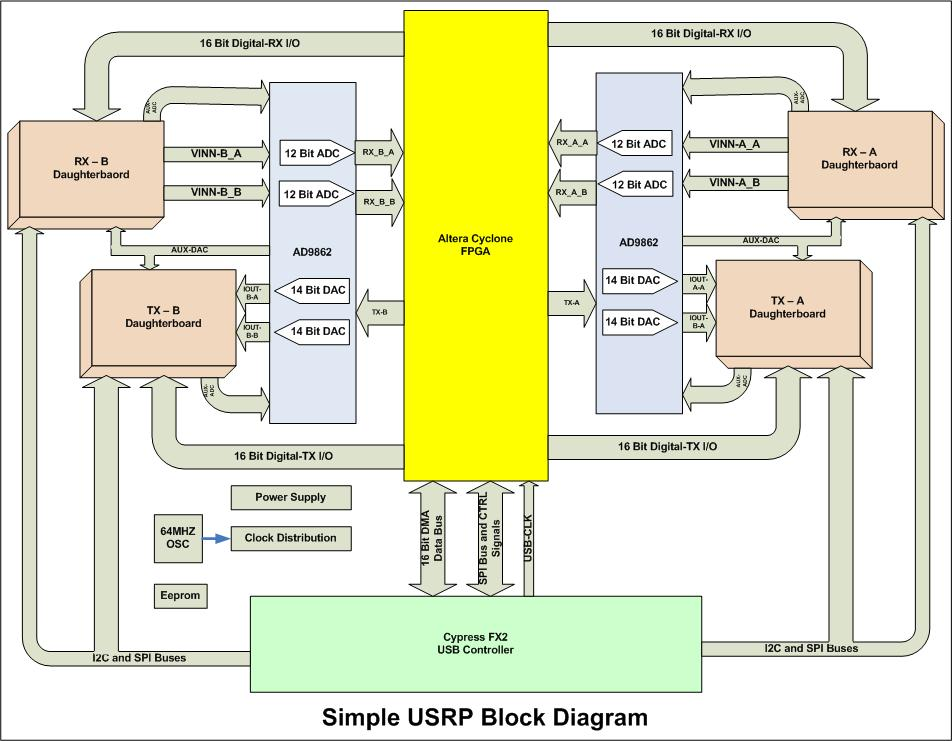
\includegraphics[scale=.6]{usrpblockdkmyg9.jpg}
\caption[Simplified USRP Block Diagram]{Simplified USRP Block Diagram}
\label{fig:usrpblock}
\end{figure}

The software radio hardware will be the Ettus Research USRP (also known as the USRP1) with two DBSRX2 receiver daughter modules each connected to a VERT900 whip antenna.

\bigskip

The connection from the URSP to the host computer is effected using a USB2 link.

\begin{figure}
\centering 
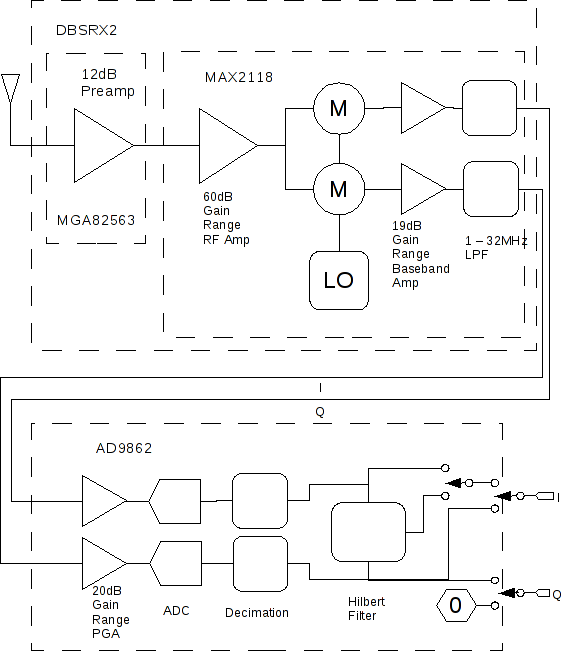
\includegraphics{Passive-Weather-Radar-Theory-fig-07.png}
\caption[Simplified Signal Path Elements of One Receive Channel]{Simplified Signal Path Elements of One Receive Channel}
\label{fig:07}
\end{figure}

\subsection[USB Interface Bandwidth]{USB Interface Bandwidth}
\label{sub:USB1}
Due to the limited bandwidth of the USB 2.0 data channel and the relatively small capacity of the on board USRP data buffers, there is a limit to the number of receive samples that can be transfered from the USRP to the host computer per unit time. In fact the baseband bandwidth is limited by the USB data rate.

\bigskip

An effective baseband bandwidth may be synthesized by making a series of observations closely spaced in time at various frequency offsets.

\bigskip

The achievable data transfer rate on a USB 2.0 link is 53 MB/s. Each sample consists of an 16 bit I and a 16 bit Q value. Therefore the USB has a capacity of approximately 13 MS/s, or a baseband bandwidth of 6.5 MHz.

\subsection[USRP FPGA]{USRP FPGA}
\label{sub:FPGA1}
The USRP uses an Altera \textit{Cyclone EP1C12Q240C8} FPGA to control the various operations. The relevant characteristics of this device are given in table \ref{tab:01}. As can be seen this device has very limited logic capabilities and memory. In addition the lack of multipliers severely limit the use of this device for signal processing.

\begin{table}
\begin{center}
\begin{tabular}{|c|c|}
\hline
Logic elements & 12060 \\ \hline
Memory bits & 239616 \\ \hline
Phase Locked Loops & 2 \\ \hline
Multipliers & 0 \\ \hline
\end{tabular}
\caption{Significant FPGA characteristics}
\label{tab:01}
\end{center}
\end{table}

\section[Design Constrains]{Design Constrains}
\subsection[USB Channel Bandwidth]{USB Channel Bandwidth}
\label{sub:USB}

As noted in \ref{sub:USB1} the USB data bandwidth is about 13 MS/s which limits the baseband width to about 6.5 MHz. This encourages the design to move as much processing to the USRP FPGA in order to reduce the demands on the USB channel. If this proves impossible it may be necessary to synthesize a baseband bandwidth by making observations closely spaced in time with different local oscillator values.

\subsection[Clock Stability]{Clock Stability}

The USRP master clock provides the reference for all local oscillators in the reception chain. Therefore variations in the frequency of this clock have a potential impact on the baseband signal, especially any Doppler processing of that signal. The specified instability of the master clock is 20 ppm. Therefore the master clock may vary up to 1280 Hz from its nominal 64 MHz.

\bigskip

In this application it is not the absolute clock stability that is so important but its variation with respect to the transmitter carrier frequency. This fact suggests a possible solution to master clock stability, namely using the received direct transmission as a frequency reference in order to correct the distortions in the baseband signal.

\subsection{FPGA}

As noted in section \ref{sub:FPGA1} the FPGA has limited capability but it is desirable to move as much of the front end processing that might normally be done on the host computer into the USRP as possible with a view to reducing USB bandwidth. As a matter of priority a surgery will be made of the Verilog code to see which of it may be discarded in this application and whether discarding any code will allow processing to be moved to the FPGA.

\clearpage\setcounter{page}{1}
\chapter[Design in the Enviroment]{Design in the Enviroment}

\section[Transmitters of Opurtunity]{Transmitters of Opurtunity}

\subsection[Characteristics of Telstra Next G Transmitters]{Characteristics of Telstra Next G Transmitters}
\label{sub:Telstra}

It is proposed to use transmitters that are components of Telstra's NextG" cell phone network. This network is widely deployed in WA. Typically there is one transmitter in each town which services the surrounding district. In addition transmitters are often placed in non urban situations as in fill. Also, in urban areas, there are a number of "segmented" transmitters usually driving sector antennae 
that are tilted in the vertical plane towards the ground.

\bigskip

At this time not a lot is known about how the transmitters are modulated. However, from the license assignments the bandwidth is 9.4 MHz, or less, and the emission designator is 9M40W7WEC. The first four alpha-numeric characters of the emission designator signify the bandwidth, in this case 9.40 MHz. The next three alpha-numeric characters signify the modulation, baseband and data types, in this case unspecified modulation, multichannel digital and unspecified data content.

It is expected that the transport access methods is CDMA using DSSS. In this case it is reasonable to assume that the transmitter signal will be modulated by some maximum length sequence, similar to those generated by linear feedback shift register generators, so that the signal is a Pseudo Random Noise (PRN) stream. In that case the chip rate is probably about 9 MHz.

\bigskip

In rural areas Telstra seems to operate their transmitters on a center frequency of 884.8 MHz (lower 880.1 MHz and upper 889.5 MHz). No doubt each station uses a different spreading code so that cell phones may discriminate between the several stations that may be within RF range.

\bigskip

The details of the spreading code use to produce the PRN stream is not known but, for this application, it is no necessary to have this knowledge. It is necessary that we faithfully receive each transmitter so that it can be used as a reference for correlating received echoes. Referring to figure \ref{fig:03} this is the main function of the Reference Tracking block.

\bigskip

In section \ref{sec:Resolution} it was asserted that, from SNR and resolution point of views, white Gaussian noise is the best achievable transmitter signal. However, for any number of reasons, white Gaussian noise is not used as the spreading signal. Instead a PRN stream is used in order to produce a signal having equivalent properties, as seen in figure \ref{fig:13}, \ref{fig:08} and \ref{fig:09}.

\begin{figure}
\centering 
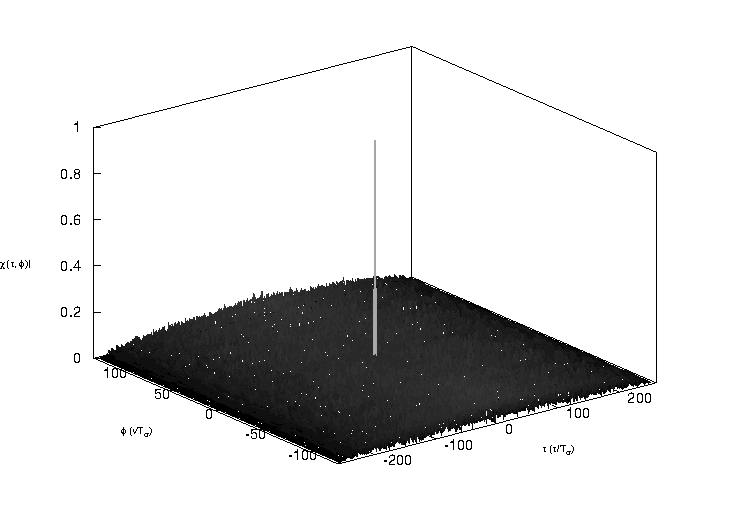
\includegraphics{Passive-Weather-Radar-Theory-fig-13.pdf}
\caption[M-Sequence ambiguity function]{M-Sequence ambiguity function}
\label{fig:13}
\end{figure}

\begin{figure}
\centering 
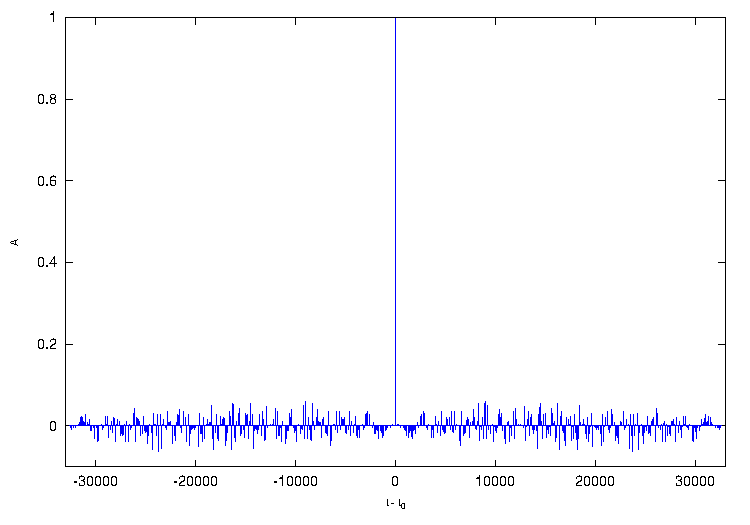
\includegraphics{Passive-Weather-Radar-Theory-fig-08.pdf}
\caption[M-Sequence autocorrelation]{M-Sequence autocorrelation}
\label{fig:08}
\end{figure}

\begin{figure}
\centering 
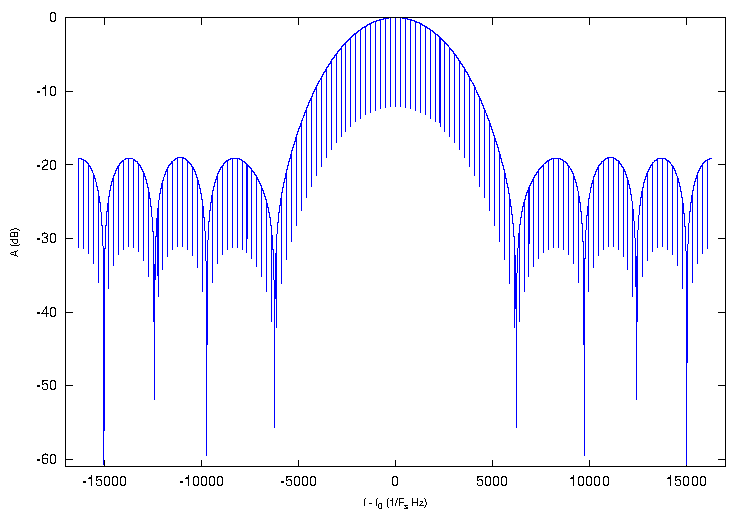
\includegraphics{Passive-Weather-Radar-Theory-fig-09.pdf}
\caption[M-Sequence envelope]{M-Sequence envelope}
\label{fig:09}
\end{figure}

\subsection[Narrogin, WA]{Narrogin, WA}

Table \ref{tab:02} lists some of the transmitters in the  Narrogin area.

\begin{table}
\begin{center}
\begin{tabular}{|p{5cm}|c|c|c|}
\hline
Site & EIRP & Position & AMG Zone 50 \\ \hline \hline
CALM Tower Williams Road Narrogin & 34.6 & S32.9383 E117.1575 & 514734 6355510 \\ \hline
Telstra Radio Terminal Wanerie & 41.1 & S33.0278 E116.8447 & 485518 6345582 \\ \hline
Western Power/Telstra Site Saunders Hill Wandering Rd Narrogin & 32.4 & S32.8942 E117.1592 & 514900 6360400 \\ \hline
Telstra CDMA Pt, North Banister & 39.9 & S32.5714 E116.4333 & 446809 6396068 \\ \hline
Telstra Radio Terminal, Mt Latham & 45 & S33.3153 E117.2769 & 625779 6313713 \\ \hline
Telstra Site Woglin Hill & 40 & S32.6781 E116.6972 & 471624 6384336 \\ \hline
Telstra Microwave Site Pingelly & 40.1 & S32.4681 E117.1014 & 509518 6407665 \\ \hline
\end{tabular}
\caption{Transmitters in the Narrogin, WA, area in frequency 884.8 MHz}
\label{tab:02}
\end{center}
\end{table}

\begin{figure}
\centering 
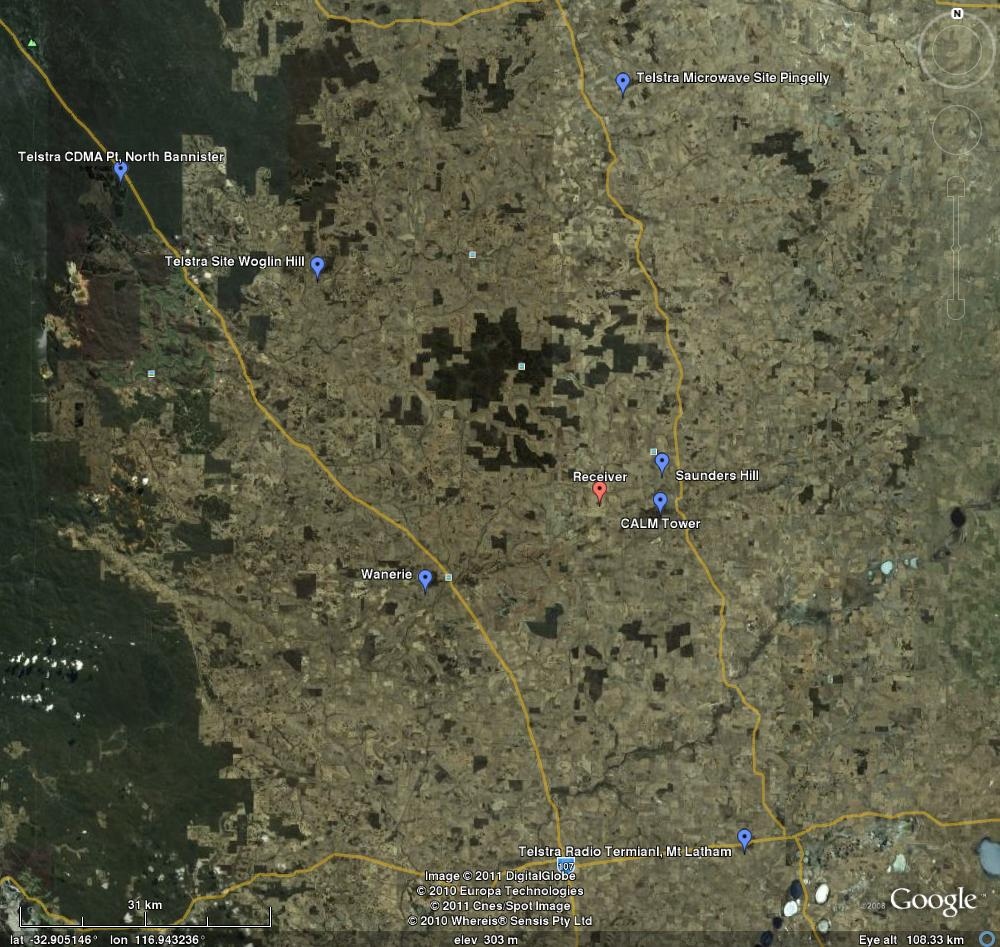
\includegraphics[scale=0.35]{Narrogin-Transmitter-Locations.jpg}
\caption[Transmitter Locations in Narrogin Area]{Transmitter Locations in Narrogin Area}
\label{fig:xmitter-Narrogin}
\end{figure}

\subsection[Melville, WA]{Melville, WA}

Table \ref{tab:03} lists some of the transmitters in the Melville area.

\begin{table}
\begin{center}
\begin{tabular}{|p{3.5cm}|c|c|c|c|}
\hline
Site & Frequency & EIRP & Position & AMG Zone 50 \\ \hline \hline
St John of God Hospital, Murdoch & 884.8 & 39.5 & S32.0689 E115.8439 & 390870 6451330 \\ \hline
St John of God Hospital, Murdoch & 2112.6 & 41.2 & S32.0689 E115.8439 & 390870 6451330 \\ \hline
St John of God Hospital, Murdoch & 2162.4 & 40.4 & S32.0689 E115.8439 & 390870 6451330 \\ \hline
St John of God Hospital, Murdoch & 2147.4 & 26.9 & S32.0689 E115.8439 & 390870 6451330 \\ \hline
K Mart North Lake Rd and South St Kardinya & 884.8 & 40.3 & S32.0686 E115.8142 & 388080 6451320 \\ \hline
K Mart North Lake Rd and South St Kardinya & 2112.6 & 44.1 & S32.0686 E115.8142 & 388080 6451320 \\ \hline
Hutchison Site 7 Rawlinson St OConnor & 885.0 & 0 & S32.0603 E115.8003 & 386753 6452212 \\ \hline
Hutchison Site 7 Rawlinson St OConnor & 2112.6 & 41.1 & S32.0603 E115.8003 & 386753 6452212 \\ \hline
\end{tabular}
\caption{Transmitters in the Melville, WA, area}
\label{tab:03}
\end{center}
\end{table}

\begin{figure}
\centering 
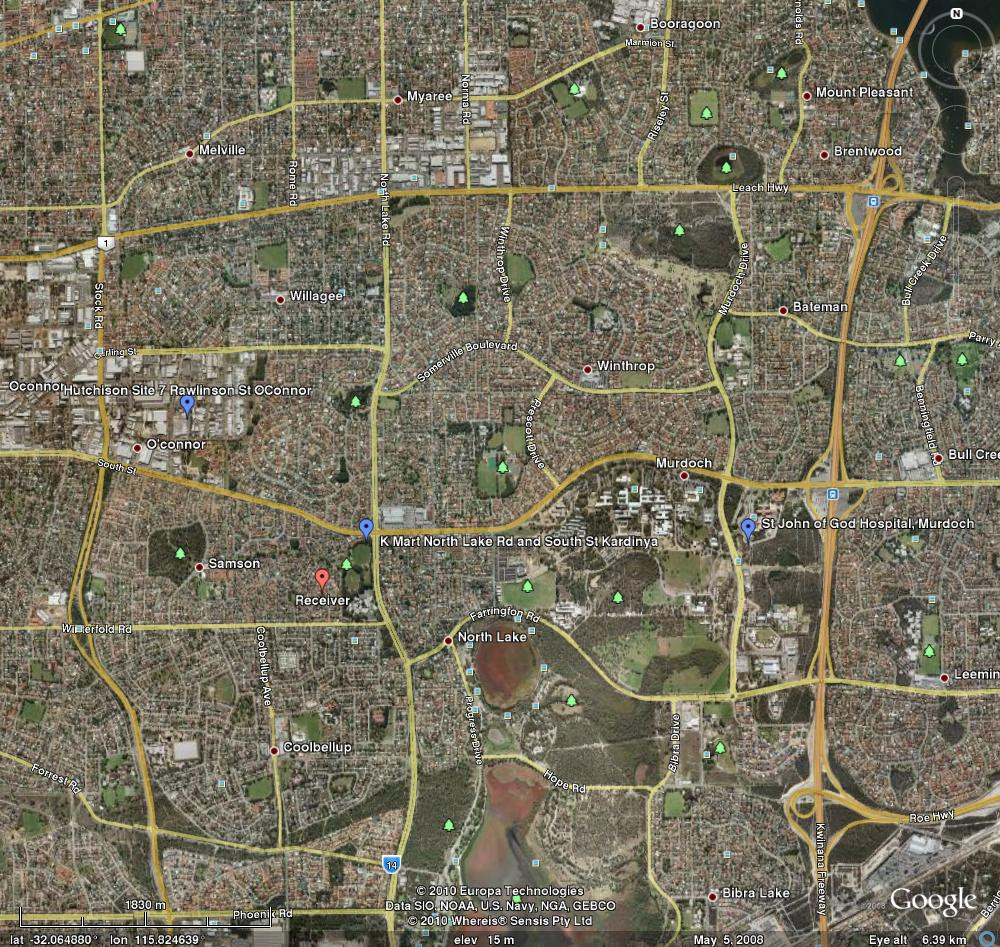
\includegraphics[scale=0.35]{Melville-Transmitter-Locations.jpg}
\caption[Transmitter Locations in Melville Area]{Transmitter Locations in Melville Area}
\label{fig:xmitter-Melville}
\end{figure}

\section[Problem of Limited Baseband Bandwidth]{Problem of Limited Baseband Bandwidth}

As mention in \ref{sub:USB} in the default configuration the USB link limits the baseband bandwidth to about 6.5 MHz. From \ref{sub:Telstra} it can be seen that the required baseband bandwidth is about 9.5 MHz. Possible solutions are:

\begin{itemize}
\item{Decimate the data in order to reduce the baseband bandwidth to about 6.5 MHz.}
\item{Transfer 8 bit samples across the USB link.}
\item{Transfer 12 bit samples across the USB link.}
\item{"Chop" the data stream.}
\end{itemize}

\bigskip

The first option will mean that the signal bandwidth will be much less that the expected bandwidth of the PRN signal. This will adversely effect the matched filter characteristics. Just as importantly the discrimination between the several transmitters relies on the ability to receive and track the PRN signal which will be adversely effected by the reduced bandwidth.

\bigskip

The second option will severely reduce the dynamic range and SNR of the system. This option may require changes to the FPGA and driver codes.

\bigskip

The third option shows promise. It is not sure why this is not done in any case. The receiver ADCs have 12 bit resolution. Packing these 12 bit samples would give a baseband bandwidth of about 9.31 MHz. For this application this bandwidth may be marginally sufficient. This option will require changes to the FPGA and driver codes.

\bigskip

The fourth option is probably the best. This option involves transmitting a block of time domain samples and then discarding a following block of samples. The size of the blocks would be such that the buffers in the FPGA and USB controller. The available buffering is about 4096 samples. From the signal processing point of view this is equivalent to multiplying the time domain signal by one corresponding to the samples transmitted and zero otherwise. As long as sample clock phase is maintained (i.e. the receiver software "knows" the number of samples dropped) then the bandwidth is equal to $F_s / 2$. However the $TB$ product is affected proportionally.

\clearpage\setcounter{page}{1}
\chapter[Project Strategy]{Project Strategy}
\section[Driving Factors]{Driving Factors}
There are a number of important factors that are unknown at this stage:
\begin{itemize}
\item{The suitability of the chosen frequency (880 Mhz) for backscatter from clouds and rain}
\item{The effect of target motion on transmitter chip rate and symbol rate and its effect on correlation}
\item{The unknown nature of the propagation model}
\item{The usefulness of the Telstra \textit{Next G} transmitters as illuminators}
\end{itemize}

\section[Implications]{Implications}
In light of the above an initial receiver consisting of a USRP with one DBSRX2 module will be built first. This will allow an investigation of the above concerns. Additionally it will allow familiarization with the hardware and its connection to the software.

\end{document}
